\chapter{存储管理}

\section{存储管理}

\subsection{存储管理}

进程调度算法能提高CPU的使用率和计算机对用户的响应速度,但是为了实现这一性能改进,必须将多个进程保存在内存中。 \\

CPU所能直接访问的存储器只有内存和寄存器,执行指令以及指令使用的数据必须在这些直接可访问的存储设备上。如果数据不在内存中,那么在CPU使用前必须先把数据移到内存中。 \\

为了确保每个进程都有独立的内存空间,通过基地址寄存器(base register)和界限地址寄存器(limit register)可以确定进程可访问的合法地址和范围。

\begin{figure}[H]
	\centering
	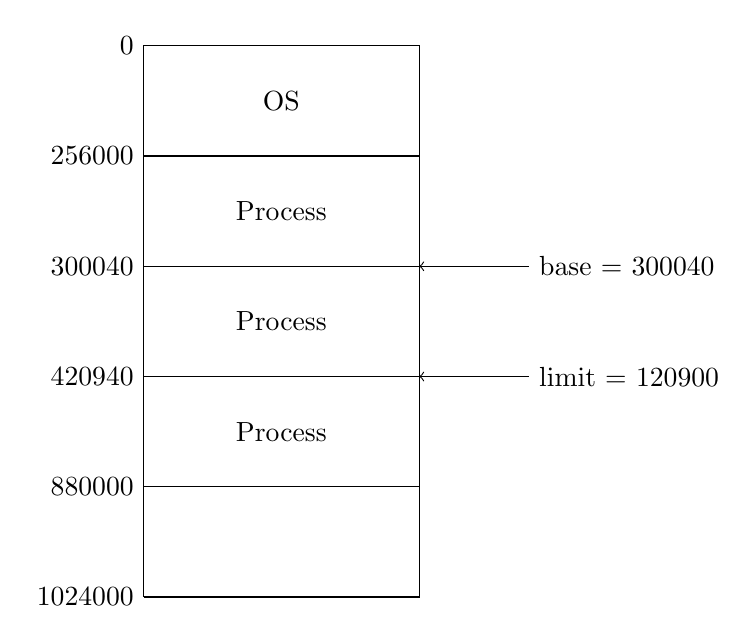
\begin{tikzpicture}[scale=0.7]
		\draw[-] (0,0) -- (0,10) -- (5,10) -- (5,0) -- (0,0);
		\draw[-] (0,2) -- (5,2);
		\draw[-] (0,4) -- (5,4);
		\draw[-] (0,6) -- (5,6);
		\draw[-] (0,8) -- (5,8);

		\draw (0,10) node[left] {0};
        \draw (0,8) node[left] {256000};
        \draw (0,6) node[left] {300040};
        \draw (0,4) node[left] {420940};
        \draw (0,2) node[left] {880000};
		\draw (0,0) node[left] {1024000};

		\draw (2.5,9) node {OS};
        \draw (2.5,7) node {Process};
		\draw (2.5,5) node {Process};
		\draw (2.5,3) node {Process};

        \draw[<-] (5,6) -- (7,6) node[right]{base = 300040};
        \draw[<-] (5,4) -- (7,4) node[right]{limit = 120900};
	\end{tikzpicture}
	\caption{基地址寄存器与界限地址寄存器}
\end{figure}

\subsection{逻辑地址与物理地址}

CPU所生成的地址为逻辑地址(logical address),而内存单元所看到的地址为物理地址(physical address)。 \\

用户程序不会看到真正的物理地址,只有当它作为内存地址时,它才进行相对于基地址寄存器的重定位,将逻辑地址转变为物理地址。

\begin{figure}[H]
	\centering
	\begin{tikzpicture}[scale=0.7]
        \draw[-] (-7,2) -- (-5,2) -- (-5,4) -- (-7,4) -- (-7,2);
        \draw (-6,3) node[]{CPU};

		\draw[-] (-1,0) -- (-1,7) -- (5,7) -- (5,0) -- (-1,0);
        \draw (2,6) node[]{Relocation Register};

        \draw[-] (10,-2) -- (10,9) -- (14,9) -- (14,-2) -- (10,-2);
        \draw (12,3.5) node[]{Memory};

        \draw[->] (-5,3) -- (-1,3);
        \draw (-3,3) node[above]{logical address};
        \draw (-3,3) node[below]{346};

        \draw (2,3) node[]{+ 14000};

        \draw[->] (5,3) -- (10,3);
        \draw (7.5,3) node[above]{physical address};
        \draw (7.5,3) node[below]{14346};
	\end{tikzpicture}
	\caption{逻辑地址与物理地址}
\end{figure}

\newpage

\section{分区}

\subsection{固定分区(Fixed Partition)}

最简单的内存分配方法之一就是将内存分为多个固定大小的分区,每个分区只能容纳一个进程。当一个分区空闲时,可以从输入队列中选择一个小于等于分区尺寸的进程调入到空闲分区。当进程终止时,其分区可以被其它进程所使用的。 \\

固定分区的好处在于实现简单、系统开销小,但是由于分区尺寸和数目固定,系统无法运行大程序,使活动进程的数目受限。同时固定分区会产生内部碎片(internal fragmentation),存储利用率不高。 \\

内部碎片的产生是由于无论进程的尺寸有多大,都会占用一个分区的空间,这样就会产生内部碎片。这部分内存在分区内,但又不能被其它进程所使用的。

\subsection{可变分区(Dynamic Partition)}

当有新进程需要内存时,为该进程查找足够大的块,如果找到,则为其分配所需的内存。 \\

这种方法属于动态存储分配问题,有三种最为常用的解决方法:

\begin{enumerate}
    \item 首次适应(first-fit):分配第一个足够大的块,每次查找从头或者从上一次首次适应结束的位置开始,一旦找到足够大的空间,就分配给进程。
    
    \item 最佳适应(best-fit):查找整个列表,分配最小的足够大的块,这种方法可以产生最小的外部碎片。
    
    \item 最差使用(worst-fit):查找整个列表,分配最大的块,这种方法可以产生最大的外部碎片。
\end{enumerate}

可变分区为进程分配了大小合适的分区,消除了内部碎片,但是却产生了外部碎片(external fragmentation)。随着进程装入和移出内存,空闲内存空间被分为小片段。当所有总的可用内存之和可以满足请求,但不连续时,就会产生外部碎片问题。 \\

为了使外部碎片得到充分利用,利用紧凑技术(compaction)可以将内存中的所有空闲分区拼接成一个较大的空闲分区。即系统可以把内存中的所有进程移到内存的某一段,那么所有空闲分区将会移到内存的另一端。

\newpage

\section{虚拟内存}

\subsection{虚拟内存(Virtual Memory)}

普通的内存管理策略都需要在进程执行之前将整个进程放在内存中,虚拟内存技术运行执行进程不必完全在内存中。这种方案的一个显著的优点就是用户会感觉到系统的内存空间比实际内存大,这种技术允许程序员不受内存存储的限制,虚拟内存也允许进程很容易地共享文件和地址空间。但是虚拟内存的实现并不容易,如果使用不当可能会极大降低性能。 \\

操作系统为每个进程分配了一套独立的虚拟地址,互不干涉,但是每个进程都不能访问物理地址。操作系统会提供一种机制,将不同进程的虚拟地址和不同内存的物理地址映射起来。如果程序要访问虚拟地址的时候,由操作系统转换成不同的物理地址,这样不同的进程运行的时候,写入的是不同的物理地址,这样就不会冲突了。进程持有的虚拟地址会通过CPU芯片中的内存管理单元MMU来转换变成物理地址。

\begin{figure}[H]
	\centering
	\begin{tikzpicture}[scale=0.7]
        \draw[-] (-7,2) -- (-5,2) -- (-5,4) -- (-7,4) -- (-7,2);
        \draw (-6,3) node[]{CPU};

		\draw[-] (-1,0) -- (-1,7) -- (5,7) -- (5,0) -- (-1,0);
        \draw (2,6) node[]{内存管理单元};

        \draw[-] (10,-2) -- (10,9) -- (14,9) -- (14,-2) -- (10,-2);
        \draw (12,3.5) node[]{物理内存};

        \draw[->] (-5,3) -- (-1,3);
        \draw (-3,3) node[above]{虚拟地址};

        \draw (2,3) node[]{MMU};

        \draw[->] (5,3) -- (10,3);
        \draw (7.5,3) node[above]{物理地址};
	\end{tikzpicture}
	\caption{虚拟内存}
\end{figure}

\newpage

\section{分段}

\subsection{分段(Segmentation)}

程序是由若干个逻辑分段组成的,如可由代码分段、数据分段、栈段、堆段组成。分段是一个支持用户视角的内存管理技术,基于模块化开发时,程序员根据需要将进程分割成许多大小不一定相同的段(segment),系统则将物理内存动态划分成许多尺寸不一定相等的分区(partition)。当一个进程被装入物理内存时,系统将为该进程的每个段独立地分配一个分区,同一进程的多个段不必存放在连续的多个分区中。 \\

段表(segment table)用于描述进程的分段情况,记载进程的各个段到物理内存中分区的映射情况。段表的基本元素包括段号、段的物理起始地址和段长度。

\begin{figure}[H]
	\centering
	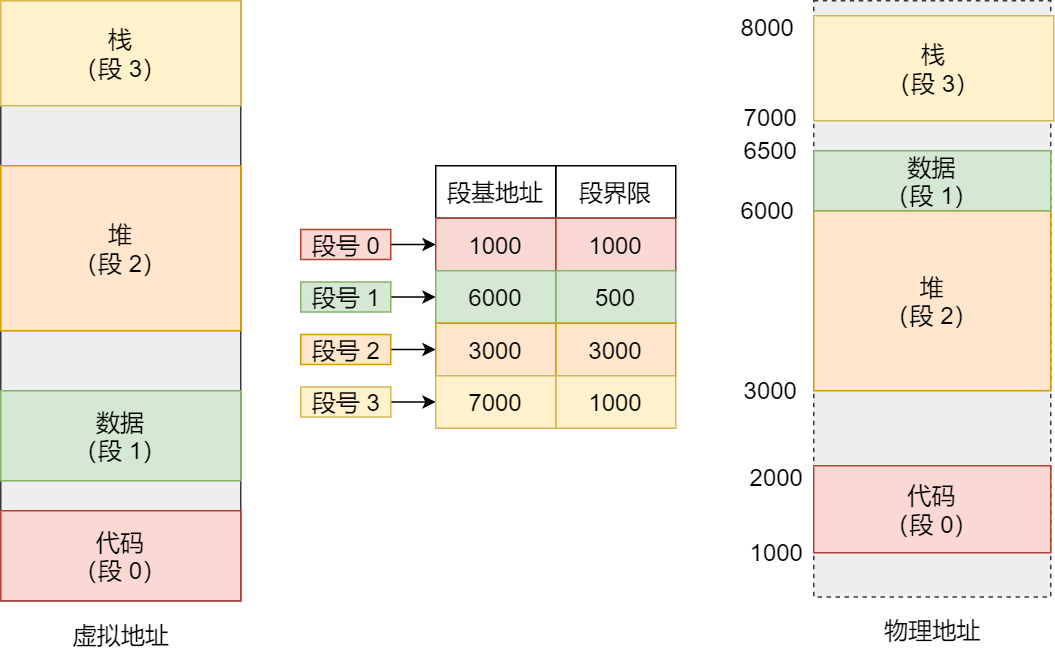
\includegraphics[scale=0.35]{img/C3/3-4/1.png}
	\caption{段表}
\end{figure}

通常,在编译程序时,编译器会自动根据程序来构造段。例如一个C编译器可能会创建代码、全局变量、堆、每个线性采用的栈、标准库函数等一系列段。在编译时链接的库可能被分配不同的段。加载程序会装入所有这些段,并为它们分配段号。 \\

分段解决了程序本身不需要关心具体的物理内存地址的问题,但它也有一些不足之处,如内存碎片和内存交换的低效率问题。

\begin{figure}[H]
	\centering
	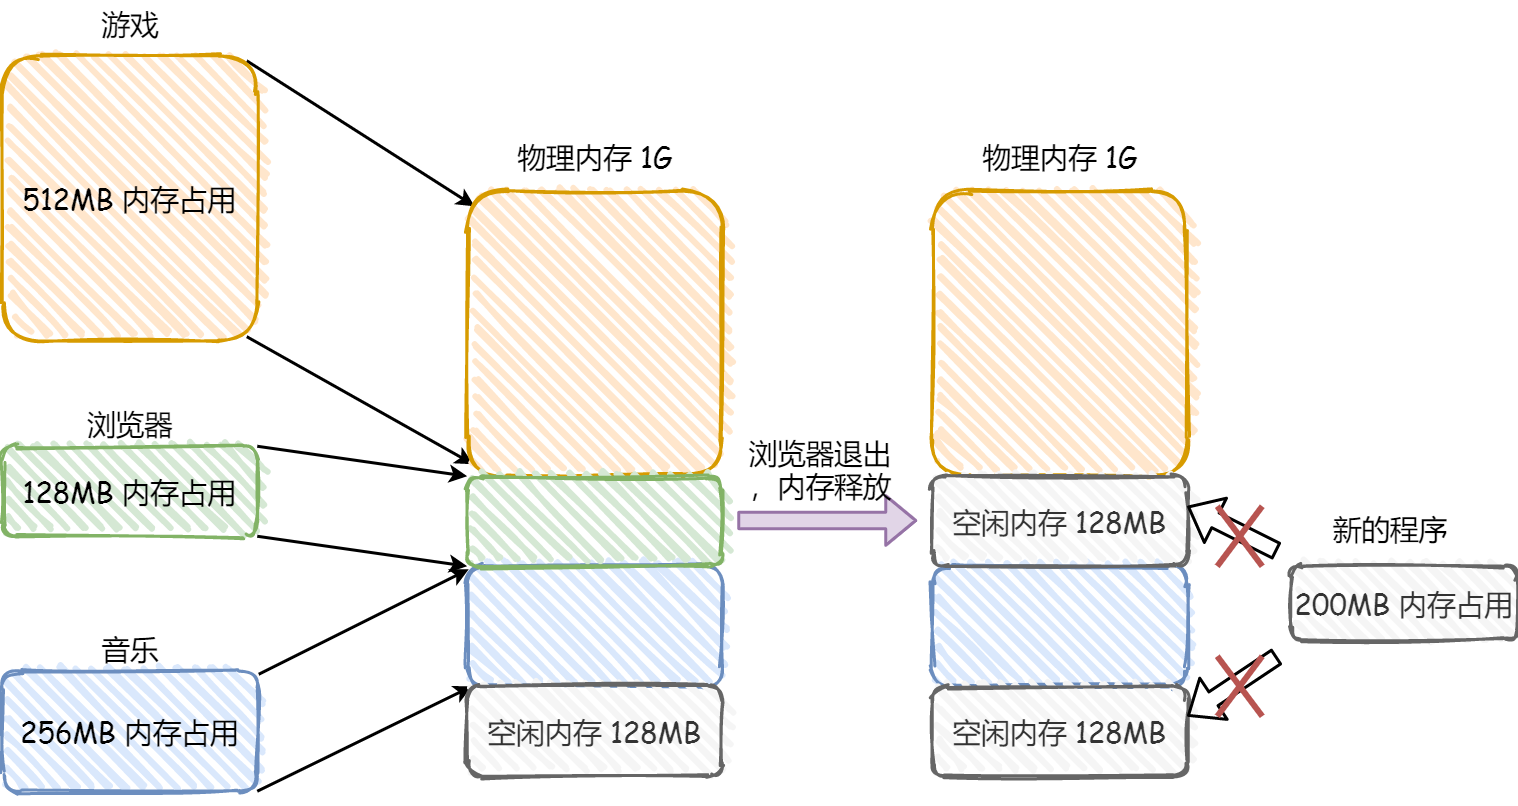
\includegraphics[scale=0.25]{img/C3/3-4/2.png}
	\caption{内存碎片}
\end{figure}

这里的内存碎片的问题共有两处地方:

\begin{enumerate}
    \item 1. 外部碎片:产生了多个不连续的物理内存,导致新的进程无法被装载。
    
    \item 内部碎片:程序所有的内存都被装载到了物理内存,但是这个程序有部分的内存可能并不是很常使用,这也会导致内存的浪费。
\end{enumerate}

解决外部内存碎片的问题就是内存交换。可以把音乐进程占用的256MB内存写到硬盘上,然后再从硬盘上读回到内存里。不过再读回的时候不能装载回原来的位置,而是紧紧跟着那已经被占用了的512MB内存后面。这样就能空缺出连续的256MB空间,于是新的200MB进程就可以装载进来。 \\

对于多进程的系统来说,分段很容易产生内存碎片,内存交换的过程就会产生性能瓶颈。因为硬盘的访问速度要比内存慢太多了,每一次内存交换,都需要把一大段连续的内存数据写到硬盘上。

\newpage

\section{分页}

\subsection{分页(Paging)}

分页内存管理方案允许进程的物理地址空间可以是非连续的。分页的基本方法是将程序分成等长的小块,称为页(page),同样内存也被分成了和页面同样大小的页框/帧(frame),这样一个页就可以装到一个页框中。 \\

分页机制把进程散布在不同的页框中,因此在执行程序的时候,需要根据页表(page table)查找某个页面在内存的某个页框中,由此完成逻辑地址到物理地址的映射。 \\

每当进程的某一条指令要访问进程内某地址时,其产生的地址都会被分割成页号和偏移量的形式。CPU根据页号查找页表,找到物理内存中该页对应的页框号用来替换页号,重新拼接成真正的物理地址。

\begin{figure}[H]
	\centering
	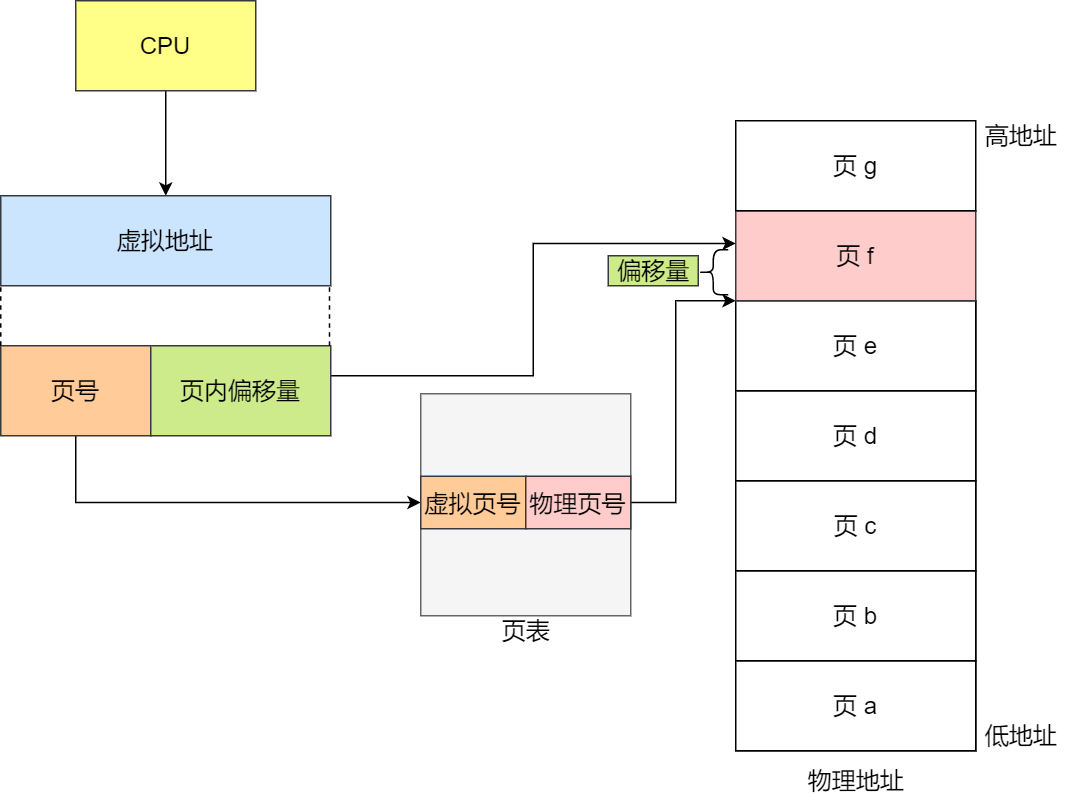
\includegraphics[scale=0.35]{img/C3/3-5/1.png}
	\caption{分页内存管理}
\end{figure}

\begin{figure}[H]
	\centering
	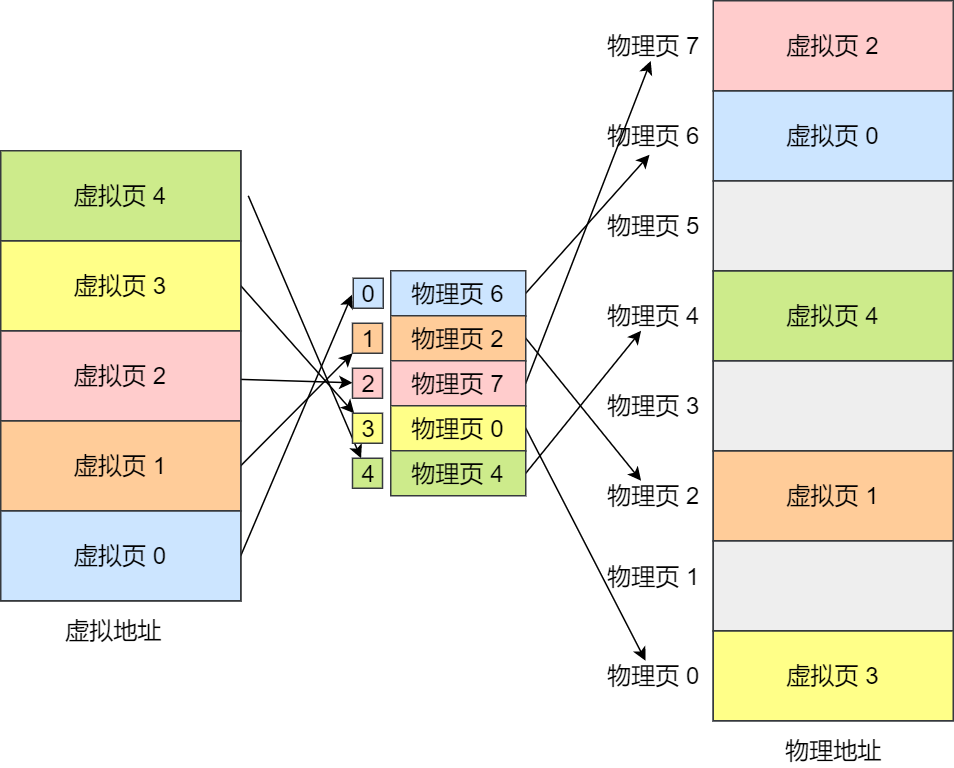
\includegraphics[scale=0.4]{img/C3/3-5/2.png}
	\caption{虚拟页与物理页}
\end{figure}

采用分页技术不会产生外部碎片,每个页框都可以分配给需要它的进程。不过,分页会产生内部碎片,如果进程所要求的内存并不是页的整数倍,那么最后一个页框就可能用不完。 \\

分页的一个重要特点是用户视角的内存和实际的物理内存是分离的,逻辑地址需要通过映射转变成物理地址,这种映射由操作系统所控制,用户是不知道的。 \\

由于内存空间都是预先划分好的,也就不会像分段会产生间隙非常小的内存。同时内存也都是以页为单位释放的,也就不会产生无法给进程使用的小内存。 \\

如果内存空间不够,操作系统会把其它正在运行的进程中的最近没被使用的内存页面暂时换出(swap out)到硬盘上。一旦需要的时候,再换入(swap in)加载进来。因此,一次性写入磁盘的也只有少数的一个页或者几个页,不会花太多时间,内存交换的效率就相对比较高。

\begin{figure}[H]
	\centering
	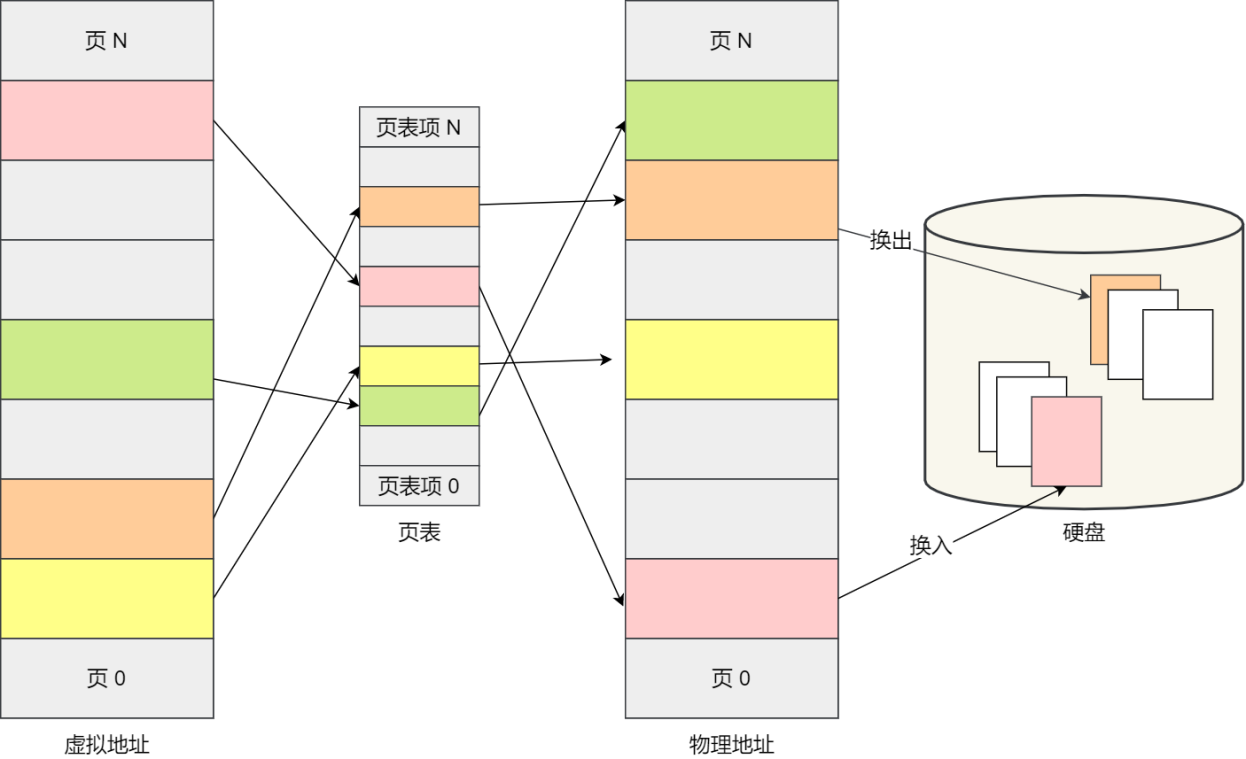
\includegraphics[]{img/C3/3-5/3.png}
	\caption{页面置换}
\end{figure}

分页的方式使得在加载程序的时候,不再需要一次性都把程序加载到物理内存中。而是只有在程序运行中,需要用到对应虚拟内存页里面的指令和数据时,再加载到物理内存里面去。

\subsection{TLB(Translation Lookaside Buffer)}

程序局部性原理是指CPU访问存储器时,无论是存取指令还是存取数据,所访问的存储单元都趋于聚集在一个较小的连续区域中。即在一段时间内,整个程序的执行仅限于程序中的某一部分。相应地,执行所访问的存储空间也局限于某个内存区域。 \\

利用这一特性,可以把最常访问的几个页表项存储到访问速度更快的硬件,于是计算机科学家们就在CPU芯片中加入了一个专门存放程序最常访问的页表项的Cache,通常称为TLB、页表缓存、快表等。有了TLB后,那么CPU在寻址时会先查TLB,如果没找到,才会继续查常规的页表。

\begin{figure}[H]
	\centering
	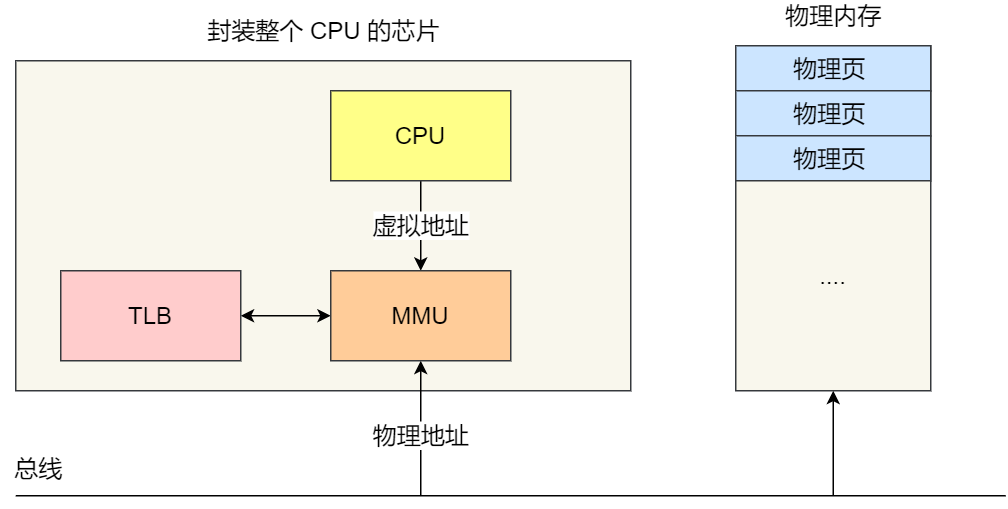
\includegraphics[scale=0.4]{img/C3/3-5/4.png}
	\caption{页面置换}
\end{figure}

\newpage


\section{页面置换算法}

\subsection{最优页面置换算法(OPT)}

当出现缺页异常,需调入新页面而内存已满时,置换算法选择被置换的物理页面。页面置换算法的设计目标是尽可能减少页面的调入调出次数,把未来不再访问或短期内不访问的页面调出。 \\

当一个缺页中断发生时,把将来最长时间不需要的页面置换。这只是一种想的情况,在实际的系统中是无法实现的,因为操作系统无法知道每一个页面要等待多长时间以后才会再次被访问。该算法无法实现,但是会利用该算法作为参考,评价其它算法。

